\begin{figure}[ht]
\tikzsetnextfilename{fractional_flow_wrt_viscosity_ratio}
\centering
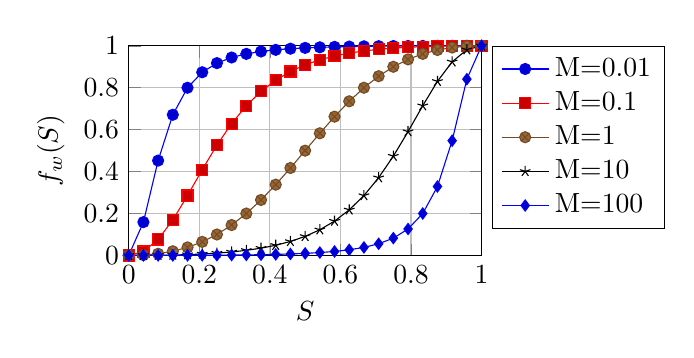
\begin{tikzpicture}
\begin{axis}[
	width=0.5\textwidth,
	height=0.35\textwidth,
	xlabel={$S$},
	ylabel={$f_w(S)$},
	xmin = 0,
	xmax = 1,
	ymin = 0,
	ymax = 1,
	domain = 0:1,
	%samples = 100,
	grid = major,
	legend style={
		cells={anchor=west},
		legend pos=outer north east,
	}
	]
	\addplot {x^2/(x^2+0.01*(1-x)^2)};
	\addplot {x^2/(x^2+0.1*(1-x)^2)};
	\addplot {x^2/(x^2+1*(1-x)^2)};
	\addplot {x^2/(x^2+10*(1-x)^2)};
	\addplot {x^2/(x^2+100*(1-x)^2)};
	\legend{M=0.01,M=0.1,M=1,M=10,M=100}
\end{axis}
\end{tikzpicture}
\caption{The fractional water flow function $f_w$, Equation (\ref{eq:fractional_flow_function}), with quadratic $k_{rl}$ and viscosity ratio $M$, Equation (\ref{eq:viscosity_ratio}).}%
\label{fig:fractional_flow_wrt_viscosity_ratio}%
\end{figure}%